\documentclass[border=4pt]{standalone}
\usepackage{amsmath,amssymb,tikz}\usetikzlibrary{arrows.meta}
\definecolor{figB}{RGB}{31,90,166}\definecolor{figR}{RGB}{176,48,48}\definecolor{figG}{RGB}{46,125,50}\definecolor{figO}{RGB}{214,120,20}
% Same T as the SVD figure: e1 at 30 deg, e2 at 120 deg, s1 = 2, s2 = 0.8, f_k = e_k rotated by 40 deg.
\begin{document}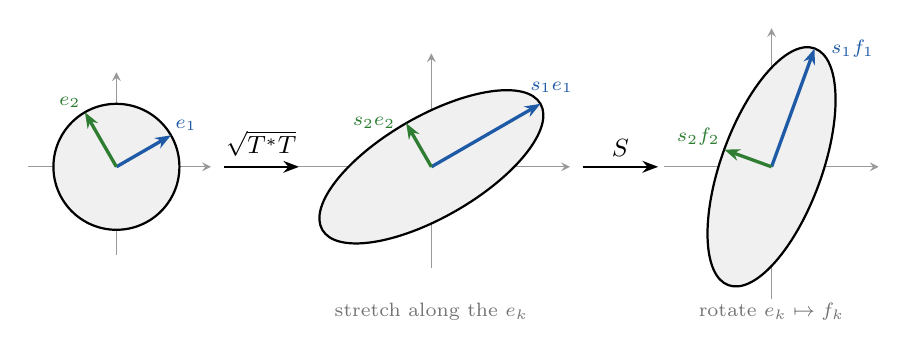
\begin{tikzpicture}[scale=0.8,>={Stealth[length=2mm]}]
\begin{scope}
\draw[black!40,thin,-stealth] (-1.4,0)--(1.5,0); \draw[black!40,thin,-stealth] (0,-1.4)--(0,1.5);
\fill[black!6] (0,0) circle (1); \draw[thick] (0,0) circle (1);
\draw[->,very thick,figB] (0,0)--(30:1) node[above right,font=\scriptsize,inner sep=1pt]{$e_1$};
\draw[->,very thick,figG] (0,0)--(120:1) node[above left,font=\scriptsize,inner sep=1pt]{$e_2$};
\end{scope}
\draw[->,thick] (1.7,0)--(2.9,0) node[midway,above,font=\small]{$\sqrt{T^*T}$};
\begin{scope}[xshift=5.0cm]
\draw[black!40,thin,-stealth] (-2.1,0)--(2.2,0); \draw[black!40,thin,-stealth] (0,-1.6)--(0,1.8);
\fill[black!6,rotate=30] (0,0) ellipse (2 and 0.8); \draw[thick,rotate=30] (0,0) ellipse (2 and 0.8);
\draw[->,very thick,figB] (0,0)--(30:2) node[above,font=\scriptsize,xshift=4pt]{$s_1e_1$};
\draw[->,very thick,figG] (0,0)--(120:0.8) node[left,font=\scriptsize]{$s_2e_2$};
\node[font=\scriptsize,black!55] at (0,-2.3) {stretch along the $e_k$};
\end{scope}
\draw[->,thick] (7.4,0)--(8.6,0) node[midway,above,font=\small]{$S$};
\begin{scope}[xshift=10.4cm]
\draw[black!40,thin,-stealth] (-1.7,0)--(1.7,0); \draw[black!40,thin,-stealth] (0,-2.1)--(0,2.2);
\fill[black!6,rotate=70] (0,0) ellipse (2 and 0.8); \draw[thick,rotate=70] (0,0) ellipse (2 and 0.8);
\draw[->,very thick,figB] (0,0)--(70:2) node[right,font=\scriptsize,xshift=2pt]{$s_1f_1$};
\draw[->,very thick,figG] (0,0)--(160:0.8) node[above left,font=\scriptsize,inner sep=1pt]{$s_2f_2$};
\node[font=\scriptsize,black!55] at (0,-2.3) {rotate $e_k\mapsto f_k$};
\end{scope}
\end{tikzpicture}\end{document}
